\chapter{Tecnologias de Transporte}

\section{PDH}

PARTE DO FÁBIO

\subsection{Multiplexação PDH}

O termo multiplexação define a tarefa de enviar dois ou mais sinais utilizando o mesmo meio de transmissão. Isso pode ser obtido de diversas maneiras, como, por exemplo, divisão do tempo de acesso ao meio em turnos para cada usuário transmitir.

Segundo \cite{Ramaswami2010}, o PDH utiliza uma multiplexação assíncrona, na qual cada terminal tem seu próprio \textit{clock}, levando a imprecisões entre as suas taxas de funcionamento, mesmo quando adotada um \textit{clock} nominal. Assim, para que haja correção nessas pequenas diferenças, deve ser inserir bits nos fluxos. Para que seja possível se captar um fluxo mais lento de informação multiplexado num fluxo mais rápido, é necessário uma estrutura chamada "montanha de multiplexadores" (ver Figura \ref{fig:muxPDH}.a), o que eleva o custo e complexidade das redes que usam esse tipo. A tabela \ref{tab:taxasPDH} mostra a nomenclatura da hierarquia de níveis de taxa de transmissão.

\begin{table}
\centering
\makebox[\textwidth][c]{
  \begin{tabular}{|l|l|l|l|l}
  \hline
  \multicolumn{2}{|c|}{América do Norte} & \multicolumn{2}{c|}{Europa}\\\hline
  Nomenclatura & Taxa de transmissão & Nomenclatura & Taxa de transmissão\\\hline
  DS0 & $0,064 \, Mb/s$ & E0 & $0,064 \, Mb/s$\\
  DS1 & $1,544 \, Mb/s$  & E1 & $2,048 \, Mb/s$\\
  DS2 & $6,312 \, Mb/s$  & E2 & $8,488 \, Mb/s$\\
  DS3 & $44,264 \, Mb/s$  & E3 & $34,368 \, Mb/s$\\
  DS4 & $139,264 \, Mb/s$  & E4 & $139,264 \, Mb/s$ \\\hline
  \end{tabular}
}
\caption{\label{tab:taxasPDH}As taxas de transmissão de sinais assíncronos e quase-síncronos (como padronizado na América do Norte e na Europa). A sigla DS vem de "\textit{Digital Signal}". Adaptado de \cite{Ramaswami2010}.}.
\end{table}

\begin{figure}
\centering
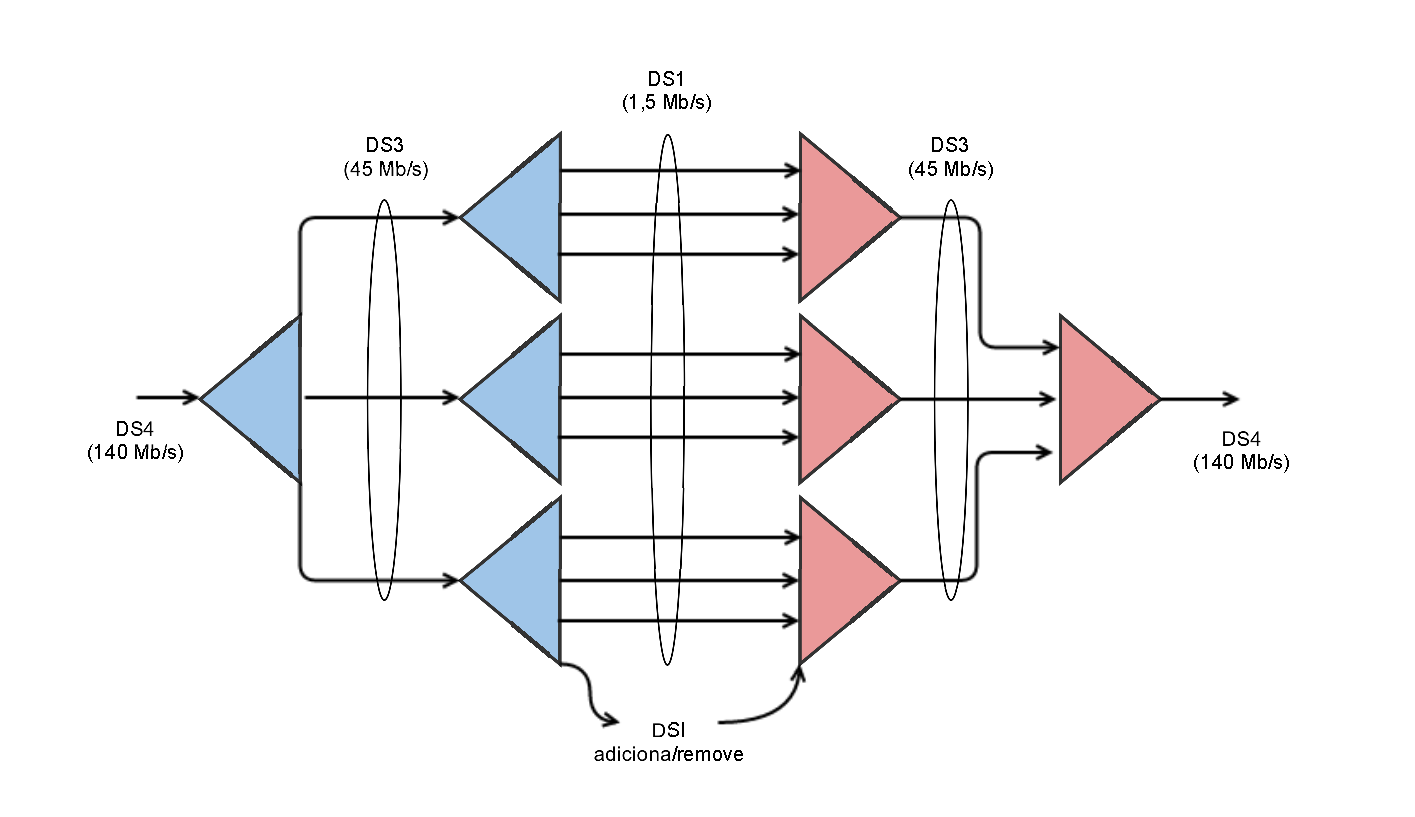
\includegraphics[width=0.9\textwidth]{image/mux_pdh.eps}
\caption{\label{fig:muxPDH} Estrutura de multiplexação PDH: a "montanha de multiplexadores". Adaptado de \cite{Ramaswami2010}.}
\end{figure}

\section{SONET}

PARTE DO FÁBIO

\subsection{Multiplexação SONET}

Ambos SONET e SDH usam métodos de multiplexação bastante sofisticados que podem ser implementados em circuitos integrados de longa escala. Comparando a figura \ref{fig:muxSDH} com a figura \ref{fig:muxPDH}, é possível notar a diferença de complexidade entre as redes SONET/SDH e PDH. Somente um componente é necessário para fazer o que a "montanha de multiplexadores" faz no PDH.

Para SONET a taxa de sinal básica é $51,84 \, Mb/s$, chamada de "\textit{synchronous transport signal level-1}" ou STS-1. As outras taxas derivadas desta são chamadas STS-N e são obtidas alternando os bytes de N  \textit{frames} STS-1 alinhados. Como os \textit{clocks} dos sinais são sincronizados, não há necessidade de inserção de bits. Por esse mesmo motivo, sinais de taxas menores podem ser extraídos de um fluxo multiplexado sem necessidade de demultiplexar o sinal inteiro. A tabela \ref{tab:taxasSONET} traz as taxas de transmissão e nomenclatura SONET.

\begin{figure}
\centering
\includegraphics[width=0.5\textwidth]{image/mux_sonet.eps}
\caption{\label{fig:muxSDH} Estrutura de multiplexação SONET. Adaptado de \cite{Ramaswami2010}.}
\end{figure}

\begin{table}
\centering
\begin{tabular}{|l|r|}
\hline
Nomenclatura & Taxa de Bit (Mb/s) \\\hline
STS-1 & $51,84$ \\
STS-3 & $155,52$ \\
STS-12 & $622,08$ \\
STS-24 & $1244,16$ \\
STS-48 & $2488,32$ \\
STS-192 & $9953,28$ \\
STS-768 & $39.814,32$ \\\hline
\end{tabular}
\caption{\label{tab:taxasSONET} As taxas de transmissão SONET e as nomenclaturas associadas às mesmas. Adaptado de \cite{Ramaswami2010}.}
\end{table}

Em SONET, os fluxos de dados de taxa inferior a STS-1 são mapeados em \textit{Virtual Tributaries} ou VTs. Os VTs são divididos em quatro tamanhos: VT1.5, VT2, VT3 e VT6, que acomodam fluxos assíncronos e plesiócronos de $1,5$, $2$, $3$ e $6 \, Mb/s$, respectivamente. Esses VTs são agrupados em um grupo VT que podem ter quatro VT1.5, três VT2, dois VT3 ou um único VT6. Cada grupo é, então, intercalado byte-a-byte junto com um junto de \textit{overheads} de caminho para formar o SONET SPE (\textit{synchronous payload envelope}) básico. A figura \ref{fig:vt} mostra graficamente como funciona a hierarquia SONET. 

Para camadas clientes (de maior abstração), como IP ou Ethernet, que tem tamanho de pacotes grandes, é usada a nomenclatura STS-Nc, em que o "c" denomina "concatenado". 

\begin{figure}
\centering
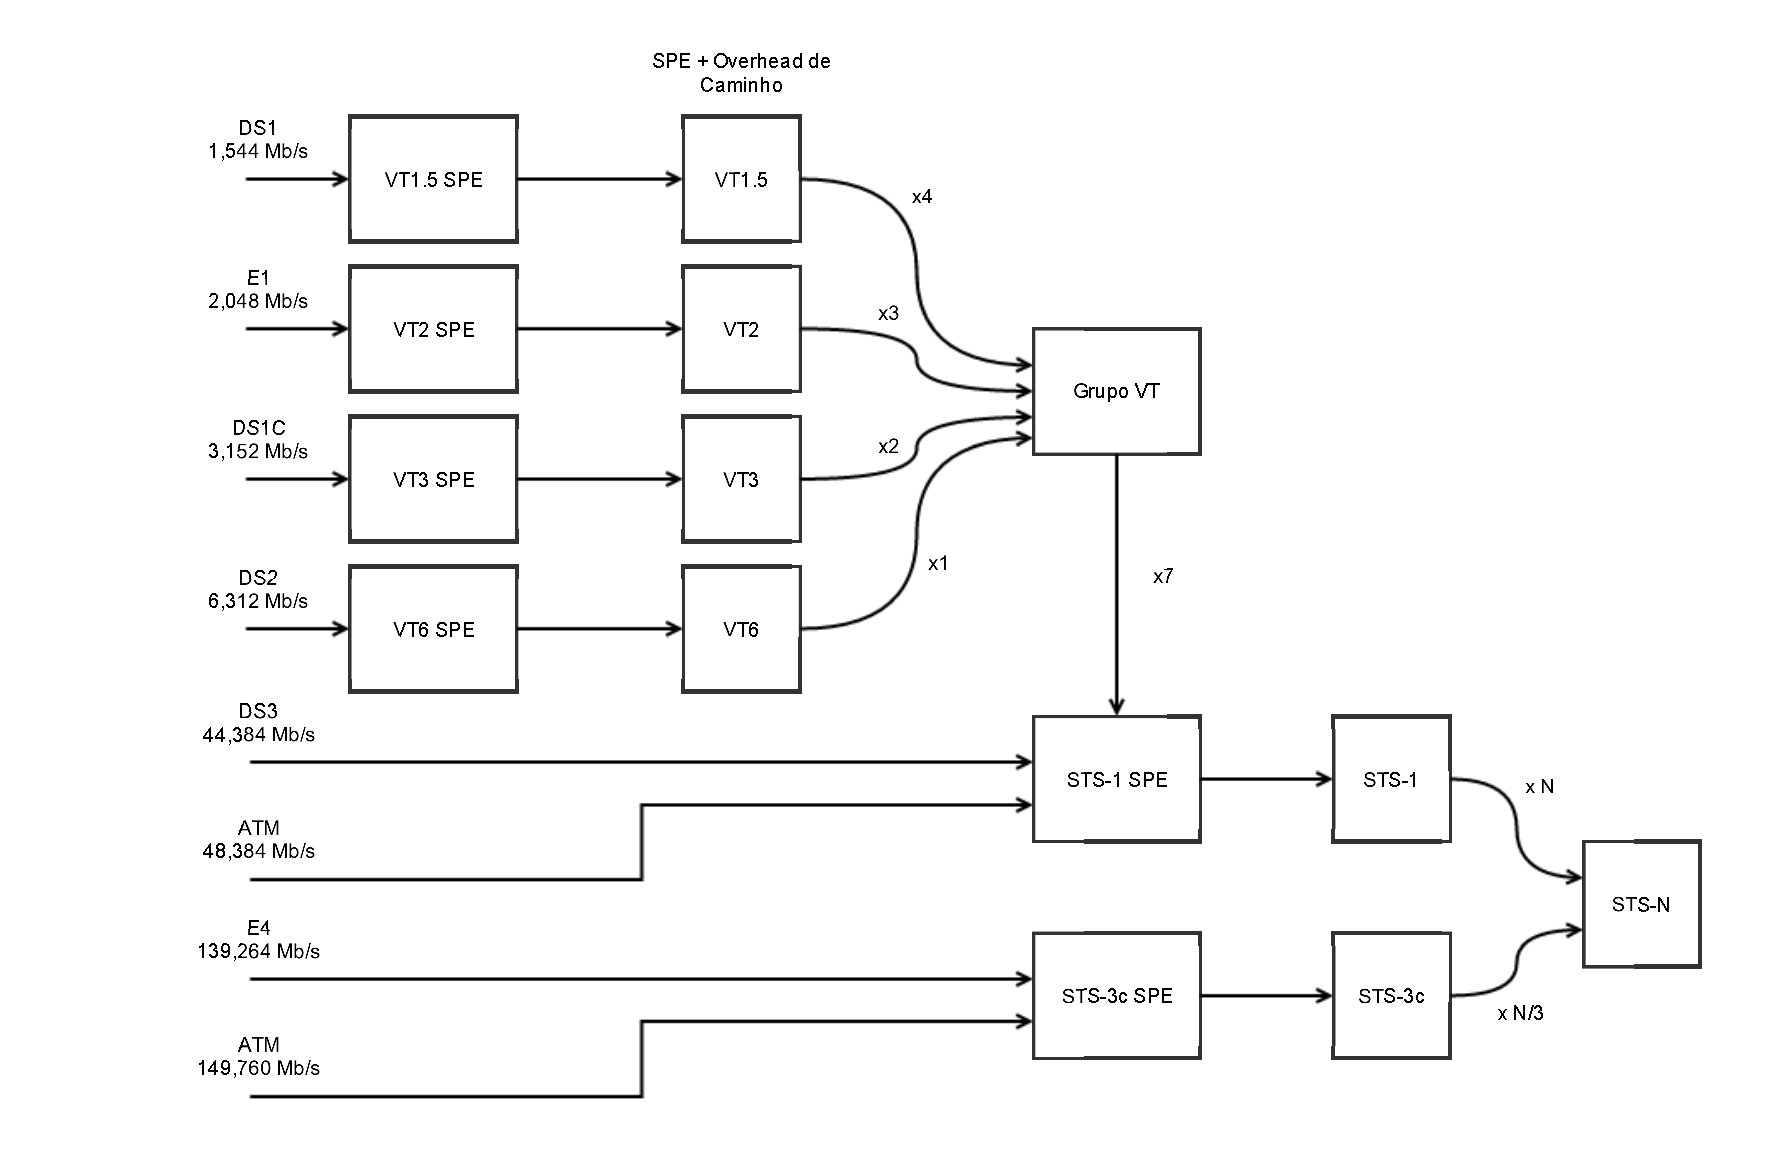
\includegraphics[width=0.9\textwidth]{image/vt.eps}
\caption{\label{fig:vt}\textit{Virtual Tributaries}. Adaptado de \cite{Ramaswami2010}.}
\end{figure}

\subsection{Multiplexação PDH}

O termo multiplexação define a tarefa de enviar dois ou mais sinais utilizando o mesmo meio de transmissão. Isso pode ser obtido de diversas maneiras, como, por exemplo, divisão do tempo de acesso ao meio em turnos para cada usuário transmitir.

Segundo \cite{Ramaswami2010}, o PDH utiliza uma multiplexação assíncrona, na qual cada terminal tem seu próprio \textit{clock}, levando a imprecisões entre as suas taxas de funcionamento, mesmo quando adotada um \textit{clock} nominal. Assim, para que haja correção nessas pequenas diferenças, deve ser inserir bits nos fluxos. Para que seja possível se captar um fluxo mais lento de informação multiplexado num fluxo mais rápido, é necessário uma estrutura chamada "montanha de multiplexadores" (ver Figura \ref{fig:muxPDH}.a), o que eleva o custo e complexidade das redes que usam esse tipo. A tabela \ref{tab:taxasPDH} mostra a nomenclatura da hierarquia de níveis de taxa de transmissão.

\begin{table}
\centering
\makebox[\textwidth][c]{
  \begin{tabular}{|l|l|l|l|l}
  \hline
  \multicolumn{2}{|c|}{América do Norte} & \multicolumn{2}{c|}{Europa}\\\hline
  Nomenclatura & Taxa de transmissão & Nomenclatura & Taxa de transmissão\\\hline
  DS0 & $0,064 \, Mb/s$ & E0 & $0,064 \, Mb/s$\\
  DS1 & $1,544 \, Mb/s$  & E1 & $2,048 \, Mb/s$\\
  DS2 & $6,312 \, Mb/s$  & E2 & $8,488 \, Mb/s$\\
  DS3 & $44,264 \, Mb/s$  & E3 & $34,368 \, Mb/s$\\
  DS4 & $139,264 \, Mb/s$  & E4 & $139,264 \, Mb/s$ \\\hline
  \end{tabular}
}
\caption{\label{tab:taxasPDH}As taxas de transmissão de sinais assíncronos e quase-síncronos (como padronizado na América do Norte e na Europa). A sigla DS vem de "\textit{Digital Signal}". Adaptado de \cite{Ramaswami2010}.}.
\end{table}

\begin{figure}
\centering
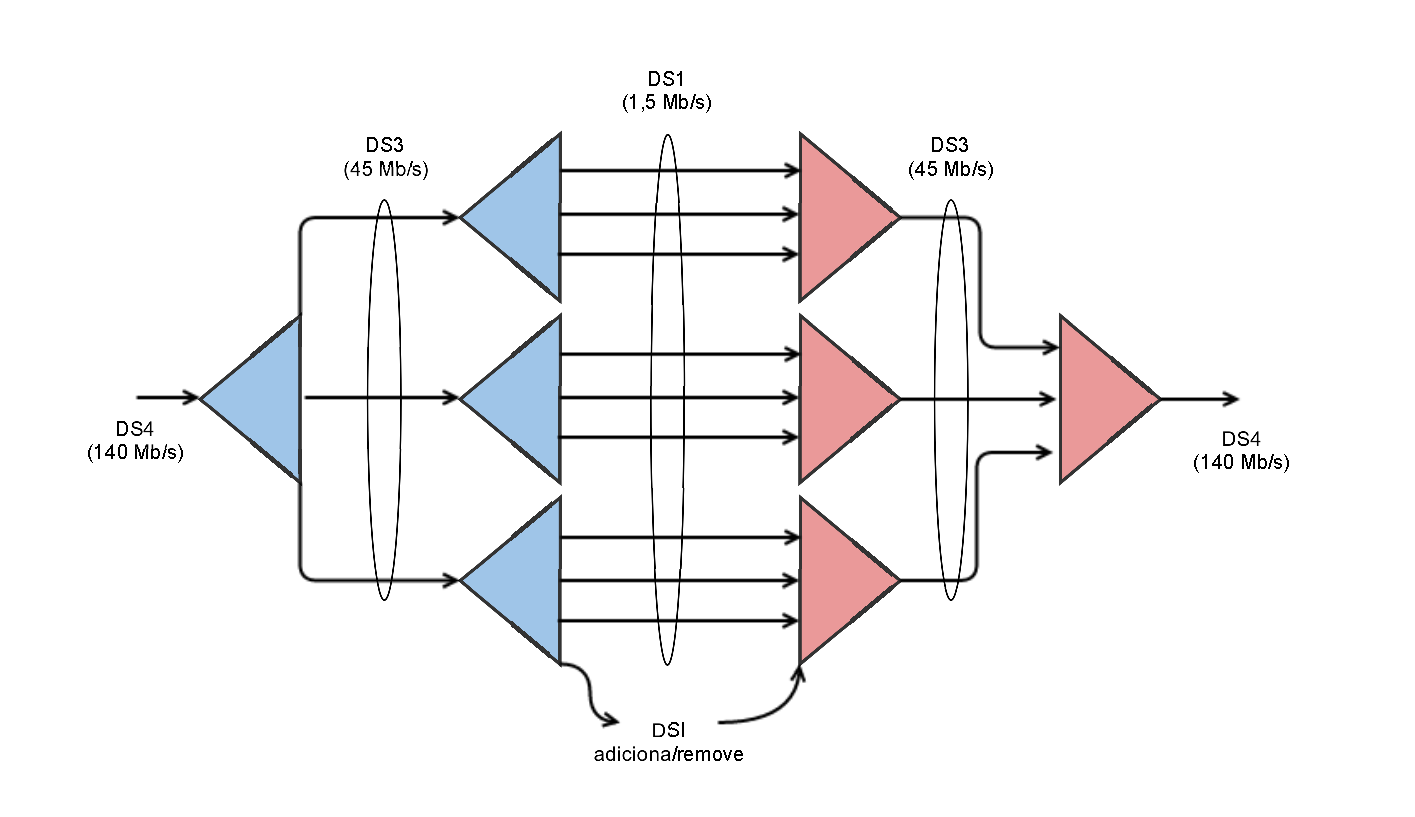
\includegraphics[width=0.9\textwidth]{image/mux_pdh.eps}
\caption{\label{fig:muxPDH} Estrutura de multiplexação PDH: a "montanha de multiplexadores". Adaptado de \cite{Ramaswami2010}.}
\end{figure}